\documentclass[tikz, border=1mm]{standalone}
\usepackage{tikz} 
\usetikzlibrary{arrows.meta}
\usepackage{pgfplots}

\begin{document}

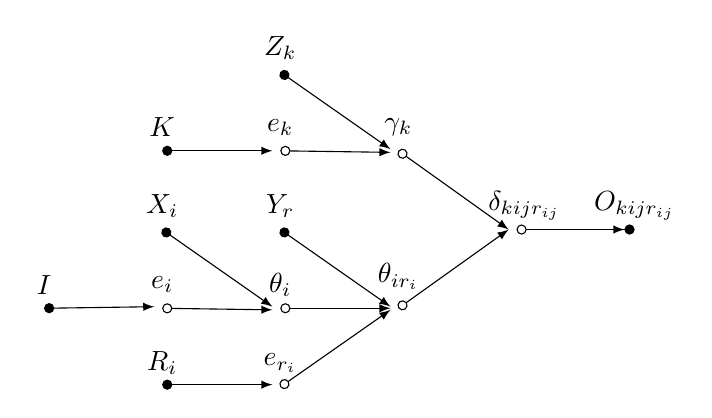
\begin{tikzpicture}

    % main graph
    % nodes
    \node at (-3,1) {$X_{i}$};
    \node at (-3,0) {$e_{i}$};
    \node at (-1.5,3) {$Z_{k}$};
    \node at (-1.5,2) {$e_{k}$};
    \node at (-1.5,1) {$Y_{r}$};
    \node at (-1.5,0) {$\theta_{i}$};
    \node at (-1.5,-1) {$e_{r_{i}}$};
    \node at (0,2) {$\gamma_{k}$};
    \node at (0,0.1) {$\theta_{ir_{i}}$};
	\node at (1.6,1) {$\delta_{kijr_{ij}}$};
    \node at (3,1) {$O_{kijr_{ij}}$};
    
	% paths
    \draw[{Circle}-{latex}](-3,0.7) to (-1.6,-0.28); % X_i -> theta_i
    \draw[{Circle[open]}-{latex}](-3,-0.3) to (-1.6,-0.32); % e_i -> theta_i
    \draw[{Circle}-{latex}](-1.5,2.7) to (-0.1,1.72); % Z_k -> gamma_k
    \draw[{Circle[open]}-{latex}](-1.5,1.7) to (-0.1,1.68); % e_k -> gamma_k
    \draw[{Circle}-{latex}](-1.5,0.7) to (-0.1,-0.28); % Y_r -> theta_ir
    \draw[{Circle[open]}-{latex}](-1.5,-0.3) to (-0.1,-0.3); % theta_i -> theta_ir
    \draw[{Circle[open]}-{latex}](-1.5,-1.3) to (-0.1,-0.32); % e_ir -> theta_ir
    \draw[{Circle[open]}-{latex}](0,1.7) to (1.4,0.7); % gamma_k -> delta_kijr
    \draw[{Circle[open]}-{latex}](0,-0.3) to (1.4,0.7); % theta_ir -> delta_kijr
    \draw[{Circle[open]}-{latex}{Circle}](1.5,0.7) to (3,0.7); % delta_kijr -> O_kijr
        
	% extras
	% nodes
    \node at (-4.5,0) {$I$}; % population of units
    \node at (-3,2) {$K$}; % population of judges
    \node at (-3,-1) {$R_{i}$}; % population of objects
    
    % paths
    \draw[{Circle}-{latex}](-4.5,-0.3) to (-3.1,-0.28); % I -> e_i
    \draw[{Circle}-{latex}](-3,1.7) to (-1.6,1.7); % K -> e_k
    \draw[{Circle}-{latex}](-3,-1.27) to (-1.6,-1.27); % R_i -> e_r(i)
    
    % X_i -> R_i
    %\draw[-{latex}](-3,0.65) to[out=180,in=85] (-5,-0.3) to[out=-95,in=180] (-3.1,-1.27); 
    
\end{tikzpicture}

\end{document}
